\documentclass[11pt]{article}
\usepackage{amsmath}
\usepackage{amssymb}
\usepackage{amsthm}
\usepackage{tikz}
\usepackage{geometry}
\geometry{margin=1in}

\DeclareMathOperator*{\argmax}{arg\,max}
% Add this next to your \argmax line
\DeclareMathOperator*{\argmin}{arg\,min}


\title{Deriving DF+L2 Loss and SF+DMD Loss with  a Simple Example}
\author{}
\date{}

\begin{document}
\maketitle

\section{Simple 2 Frame Setup}
Let's derive DF+L2 loss with simple example:

We have a two frame video: $X_1, X_2$

Each frame has a noise level:
$K \sim \text{Uniform}(0, K)$ where 0 is no noise, $K$ is full.

So $X_1^{K_1}, X_2^{K_2}$ are the two frames with their noise levels $K_1, K_2$ respectively.

\section{Diffusion Forcing Objective}
We derive a more general view of diffusion forcing objective by deriving the ELBO for the 2 frame case.

Let us define our goal:
\begin{align}
\argmax_\theta \mathbb{E}_{X_1^0, X_2^0 \sim p_{\text{data}}} \left[ \ln(p_\theta(X_1^0, X_2^0)) \right]
\end{align}

We derive a surrogate objective via the ELBO:
\begin{align}
\mathbb{E}_{X_1^0, X_2^0} \left[ \ln(p_\theta(X_1^0, X_2^0)) \right]
\end{align}

\begin{align}
= \mathbb{E}_{X_1^0, X_2^0} \left[ \ln \int p_\theta(X_1^0, X_2^0, X_1^{i:K}, X_2^{i:K}) dX_1^{i:K} dX_2^{i:K} \right]
\end{align}

Let's assume a Gaussian noising process:
\begin{align}
q(X_i^k | X_i^0) &\sim \alpha_K X_i^0 + \beta_K \epsilon, \quad \epsilon \sim \mathcal{N}(0, I) \\
&\sim \mathcal{N}(\alpha_K X_i^0, \beta_K I)
\end{align}

\begin{align}
&= \mathbb{E}_{X_1^0, X_2^0} \left[ \ln \int p(X_1^{0:K}, X_2^{0:K}) \cdot \frac{q(X_1^{1:K}, X_2^{1:K} | X_1^0, X_2^0)}{q(X_1^{1:K}, X_2^{1:K} | X_1^0, X_2^0)} dX_1^{1:K} dX_2^{1:K} \right] \\
&= \mathbb{E}_{X_1^0, X_2^0 \sim p_{\text{data}}} \left[ \ln \mathbb{E}_{X_1^{1:K}, X_2^{1:K} \sim q(\cdot | X_1^0, X_2^0)} \left[ \frac{p(X_1^{0:K}, X_2^{0:K})}{q(X_1^{1:K}, X_2^{1:K} | X_1^0, X_2^0)} \right] \right] \\
&\geq \mathbb{E}_{X_1^0, X_2^0 \sim p_{\text{data}}, X_1^{1:K}, X_2^{1:K} \sim q(\cdot | X_1^0, X_2^0)} \left[ \ln \left[ \frac{p(X_1^{0:K}, X_2^{0:K})}{q(X_1^{1:K}, X_2^{1:K} | X_1^0, X_2^0)} \right] \right]
\end{align}

\begin{align}
p(X_1^{0:K}, X_2^{0:K}) = p(X_1^K, X_2^K) \prod_{i \in \tau} p(T_{i-1} | T_i), \quad \tau \sim \text{Traj}(2,K)
\end{align}

where $T_i$ is the ith state in a trajectory, but always: $T_0 = (X_1^0, X_2^0)$, $T_K = (X_1^K, X_2^K)$.

Traj$(2, K)$ is the set of all trajectories on a 2-dimensional cube with $K$ delimiters. From 0 vertex to the opposite vertex. Note that we can construct the joint distribution in any order according to the denoising trajectories we allow, and we can assign any probability distribution over these trajectories. This flexibility allows us to model different generative processes by choosing different trajectory distributions. In the general case beyond the 2-frame example, we would replace 2 with $n$ to get Traj$(n, K)$, representing trajectories on an $n$-dimensional cube.

\begin{align}
= \mathbb{E}_{X_1^{0:K}, X_2^{0:K}} \left[ \ln p(X_1^K, X_2^K) + \sum_{T_i \in \text{Traj}(2,K)} \ln \left( \frac{p(T_{i-1} | T_i)}{q(T_i | T_{i-1})} \right) \right]
\end{align}

\begin{align}
= \mathbb{E}_{X_1^{0:K}, X_2^{0:K}} \left[ \ln p(X_1^K, X_2^K) \right] + \sum_{T_i \in \text{Traj}(2,K)} \mathbb{E}_{T_{i-1}, T_i} \left[ \ln \left( \frac{p(T_{i-1} | T_i) \cdot q(T_{i-1})}{q(T_{i-1} | T_i) \cdot q(T_i)} \right) \right]
\end{align}

We take all constants w.r.t $p$ out:
\begin{align}
\mathbb{E}_{X_1^K, X_2^K} \left[ \ln p(X_1^K, X_2^K) \right] + \sum_{T_i \in \text{Traj}(2,K)} \mathbb{E}_{T_{i-1}, T_i} \left[ \ln \left( \frac{p(T_{i-1} | T_i)}{q(T_{i-1} | T_i)} \right) \right]
\end{align}

\begin{align}
= \mathbb{E}_{X_1^K, X_2^K} \left[ \ln p(X_1^K, X_2^K) \right] - \sum_{T_i \in \text{Traj}(2,K)} D_{KL}(q(T_{i-1} | T_i) || p(T_{i-1} | T_i))
\end{align}

Note that $q(X_1^K, X_2^K) = p(X_1^K, X_2^K) = \mathcal{N}(0, I)$, and our model parameters typically do not change $p(X_1^K, X_2^K)$, so we can discard the first term. This gives us a simple sum of KL divergences over trajectories sampled from our trajectory distribution:
\begin{align}
\mathcal{L} = \sum_{\tau \sim \text{Traj}(2,K)} \sum_{i \in \tau} D_{KL}(q(T_{i-1} | T_i) || p(T_{i-1} | T_i))
\end{align}

The probabilities assigned to each trajectory should correspond to the importance of each trajectory when sampling from the model. Recall that each trajectory can be decomposed as a sequence of transitions from $T_i$ to $T_{i-1}$ (denoising steps). Our loss can also be written as an expectation over trajectory states:
\begin{align}
\mathcal{L} = \mathbb{E}_{\tau \sim \text{Traj}(2,K)} \left[ \mathbb{E}_{T_i \in \tau} \left[ D_{KL}(q(T_{i-1} | T_i) || p(T_{i-1} | T_i)) \right] \right]
\end{align}

Or equivalently as a weighted sum over all possible trajectories:
\begin{align}
= \sum_{\tau \in \text{Traj}(2,K)} p(\tau) \sum_{T_i \in \tau} D_{KL}(q(T_{i-1} | T_i) || p(T_{i-1} | T_i))
\end{align}

If we instead write this as probability distributions over atomic transitions marginalized over the distribution of trajectories, we get:

\begin{align}
= \sum_{T_i \rightarrow T_{i-1} \in \text{Traj}(2,K)} P(T_i \rightarrow T_{i-1}) D_{KL}(q(T_{i-1} | T_i) || p(T_{i-1} | T_i))
\end{align}

\section{Generalizing to the n-frame case}

To generalize to the n-frame case, we just change 2 to n.

\begin{align}
\sum_{T_i \in \text{Traj}(n,K)} P(T_i \rightarrow T_{i-1}) D_{KL}(q(T_{i-1} | T_i) || p(T_{i-1} | T_i))
\end{align}

In DF paper it applies equal probability to each transition:
\begin{align}
P(T_{i-1} \rightarrow T_i) = P(T_{j-1} \rightarrow T_j) 
\end{align}

but this should not be the case if we never double back and assign equal probability to each trajectory (you expect transitions of states near the diagonal to be weighted more by the binomial Thm).

Practically, this should not matter too much but good to keep in mind that our prior over Trajectories is not uniform (but over transitions is).

% If we asssume equal probability for each trajectory in DF, our weights should be proportional to:

% \begin{align}
% \begin{pmatrix}
% K_1 + \cdots + K_n - 1 \\
% K_1, K_2, \cdots, K_i - 1, \cdots, K_n
% \end{pmatrix} + \begin{pmatrix}
% (K - K_1) + \cdots + (K - K_n) \\
% K - K_1, \cdots, K - K_n
% \end{pmatrix}
% \end{align}

% \begin{align}
% = \begin{pmatrix}
% n \cdot K \\
% K, K, \cdots, K
% \end{pmatrix}_{n \text{ times}}
% \end{align}

Also, in an architecture like the Transformer, our state transitions decrease the noise level of each frame by 1, so the space of trajectories looks more like a diagonal pattern, but this proof still holds as we did not make any assumptions about the transitions allowed as long as they they are steadily denoising the frames.


\begin{center}
    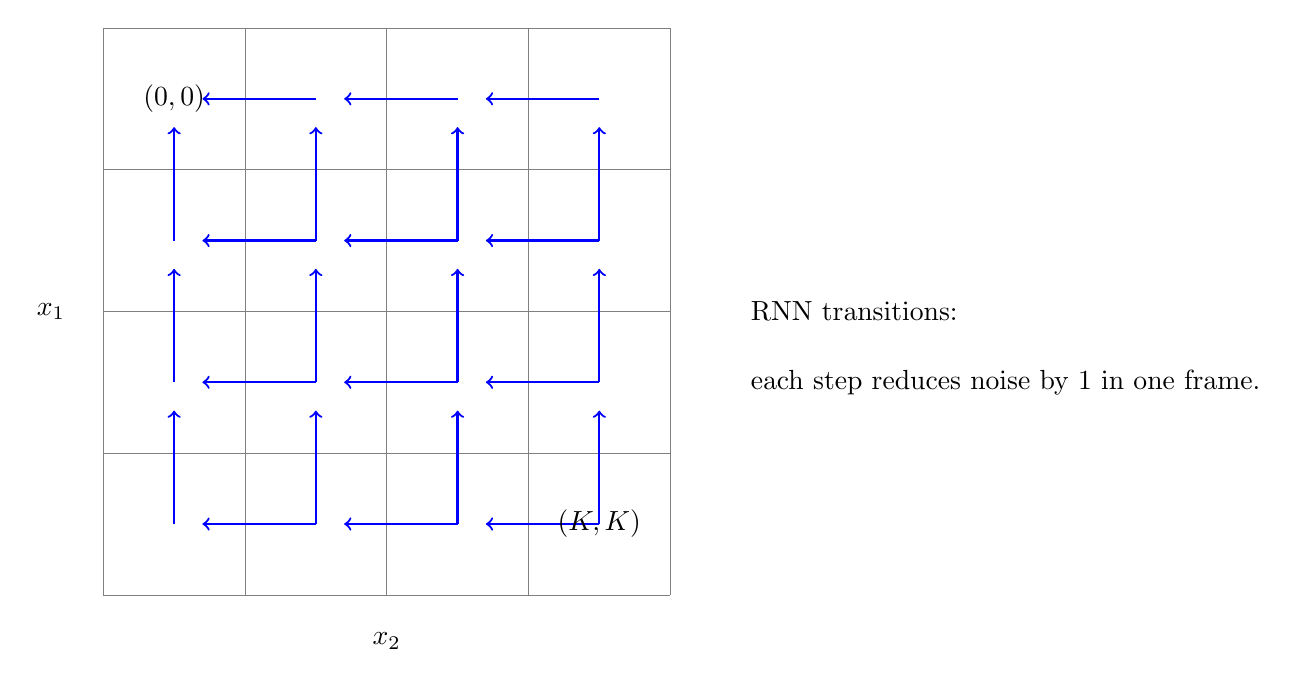
\begin{tikzpicture}[scale=1.8]
    \draw[step=1cm,gray,very thin] (0,0) grid (4,4);
    % Interior points with up and left arrows (no diagonals)
    \foreach \x in {1,2,3} {
      \foreach \y in {0,1,2} {
        \draw[->,thick,blue] (\x+0.5,\y+0.5) -- (\x-0.3,\y+0.5);
        \draw[->,thick,blue] (\x+0.5,\y+0.5) -- (\x+0.5,\y+1.3);
      }
    }
    % Left edge (only up arrows)
    \foreach \y in {0,1,2} {
      \draw[->,thick,blue] (0.5,\y+0.5) -- (0.5,\y+1.3);
    }
    % Top row (only left arrows)
    \foreach \x in {1,2,3} {
      \draw[->,thick,blue] (\x+0.5,3.5) -- (\x-0.3,3.5);
    }
    % Corner labels
    \node at (0.5,3.5) {$(0,0)$};
    \node at (3.5,0.5) {$(K,K)$};
    % Axis labels
    \node[anchor=east] at (-0.2,2) {$x_1$};
    \node[anchor=north] at (2,-0.2) {$x_2$};
    \node[anchor=west] at (4.5,2) {RNN transitions:};
    \node[anchor=west] at (4.5,1.5) {each step reduces noise by 1 in one frame.};
    \end{tikzpicture}
    \end{center}
    

\begin{center}
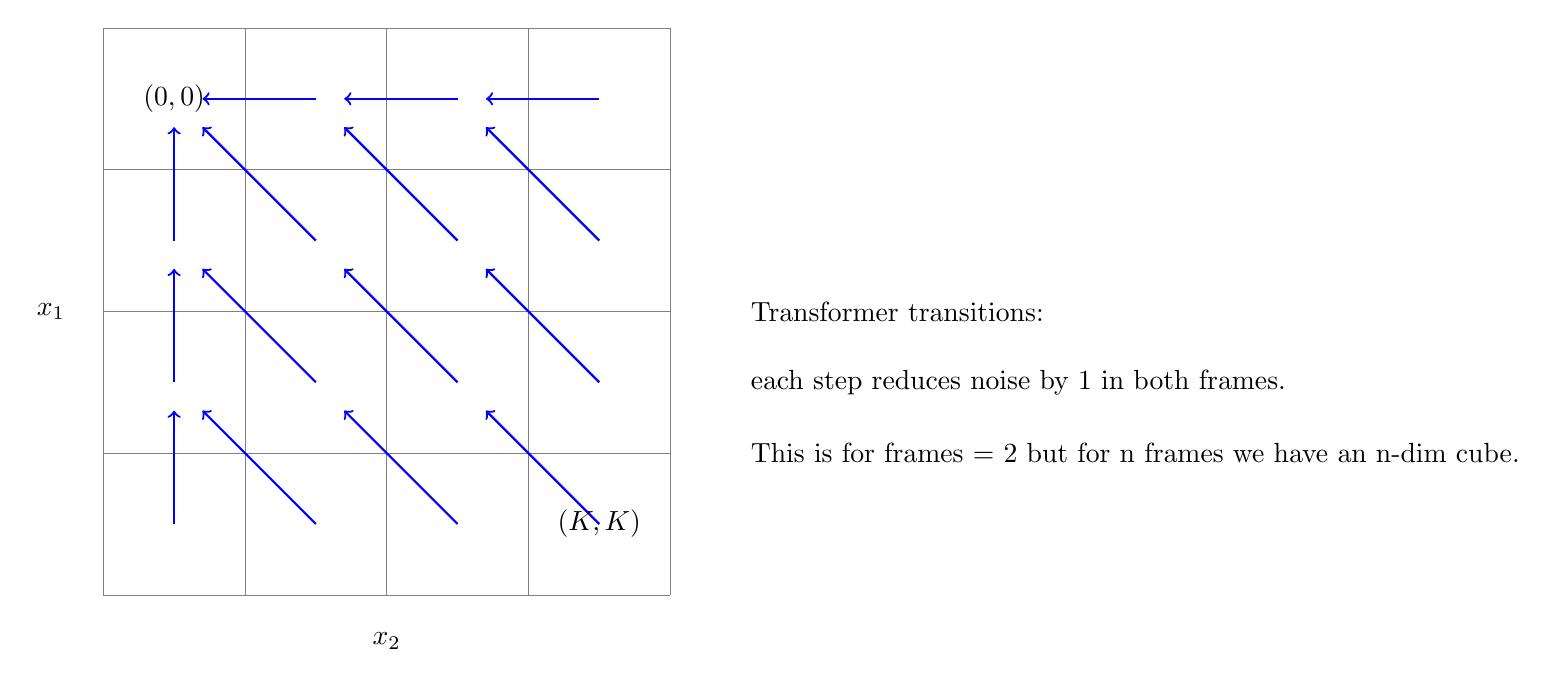
\begin{tikzpicture}[scale=1.8]
\draw[step=1cm,gray,very thin] (0,0) grid (4,4);
% Interior points with diagonal arrows (up-left)
\foreach \x in {1,2,3} {
  \foreach \y in {0,1,2} {
    \draw[->,thick,blue] (\x+0.5,\y+0.5) -- (\x-0.3,\y+1.3);
  }
}
% Left edge (only up arrows)
\foreach \y in {0,1,2} {
  \draw[->,thick,blue] (0.5,\y+0.5) -- (0.5,\y+1.3);
}
% Top row (only left arrows)
\foreach \x in {1,2,3} {
  \draw[->,thick,blue] (\x+0.5,3.5) -- (\x-0.3,3.5);
}
% Corner labels
\node at (0.5,3.5) {$(0,0)$};
\node at (3.5,0.5) {$(K,K)$};
% Axis labels
\node[anchor=east] at (-0.2,2) {$x_1$};
\node[anchor=north] at (2,-0.2) {$x_2$};
\node[anchor=west] at (4.5,2) {Transformer transitions:};
\node[anchor=west] at (4.5,1.5) {each step reduces noise by 1 in both frames.};
\node[anchor=west] at (4.5,1) {This is for frames = 2 but for n frames we have an n-dim cube.};
\end{tikzpicture}
\end{center}

\begin{center}
\begin{tikzpicture}[scale=1.8]
\draw[step=1cm,gray,very thin] (0,0) grid (4,4);
% Teacher Forcing: edge trajectory from (K,K) -> (K,0) -> (0,0)
% First go up along left edge of bottom-right corner
\draw[->,thick,blue] (3.5,0.5) -- (3.5,1.3);
\draw[->,thick,blue] (3.5,1.5) -- (3.5,2.3);
\draw[->,thick,blue] (3.5,2.5) -- (3.5,3.3);
% Then go left along top row
\draw[->,thick,blue] (3.5,3.5) -- (2.7,3.5);
\draw[->,thick,blue] (2.5,3.5) -- (1.7,3.5);
\draw[->,thick,blue] (1.5,3.5) -- (0.7,3.5);
% Corner labels
\node at (0.5,3.5) {$(0,0)$};
\node at (3.5,0.5) {$(K,K)$};
% Axis labels
\node[anchor=east] at (-0.2,2) {$x_1$};
\node[anchor=north] at (2,-0.2) {$x_2$};
\node[anchor=west] at (4.5,2) {Teacher Forcing transitions:};
\node[anchor=west] at (4.5,1.5) {denoise one frame completely,};
\node[anchor=west] at (4.5,1) {then move to the next frame.};
\end{tikzpicture}
\end{center}

TF is encapsulated in this framework too.

Like above, TF weights should be a constant traversing the edge of the cube from frame 1 $\rightarrow$ frame 2 $\rightarrow$ ... denoising which is:

\begin{align}
\mathbb{I}\left( \left\{ X_1^0, X_2^0, \ldots, X_i^{K_i}, X_{i+1}^K, \ldots, X_n^K \right\} \rightarrow \left\{ X_1^0, X_2^0, \ldots, X_i^{K_i-1}, X_{i+1}^K, \ldots, X_n^K \right\} \right)
\end{align}

i.e. pick any frame $i$, every frame to the left should be clean, every frame to the right should be full noise, and the transition should be denoising the $i$th frame by 1 noise level.


\section{Deriving the Self-Forcing Objective and Training Algorithm}

Similarly, we can derive a more general view of self forcing with DMD by deriving the ELBO for the 2 frame case.


Let's derive the self-forcing objective and training algorithm from the following:

Instead of $\argmax_\theta \mathbb{E}_{X \sim p_{\text{data}}} \left[ \ln(p_\theta(X)) \right]$,

we swap $p_{\text{data}}$ and $p_\theta$ to get:
\begin{align}
\argmax_\theta \mathbb{E}_{X_1^0, X_2^0 \sim p_\theta} \left[ \ln(p_{\text{data}}(X_1^0, X_2^0)) \right]
\end{align}

\begin{align}
= \argmax_\theta \mathbb{E}_{X_1^0, X_2^0 \sim p_\theta} \left[ \ln \int p_{\text{data}}(X_1^{0:K}, X_2^{0:K}) \cdot \frac{p_\theta(X_1^{1:K}, X_2^{1:K} | X_1^0, X_2^0)}{p_\theta(X_1^{1:K}, X_2^{1:K} | X_1^0, X_2^0)} dX_1^{1:K} dX_2^{1:K} \right]
\end{align}

\begin{align}
= \argmax_\theta \mathbb{E}_{X_1^0, X_2^0 \sim p_\theta, } \left[ \ln \mathbb{E}_{X_1^{1:K}, X_2^{1:K} \sim p_\theta(\cdot | X_1^0, X_2^0)} \left[ \frac{p_{\text{data}}(X_1^{0:K}, X_2^{0:K})}{p_\theta(X_1^{1:K}, X_2^{1:K} | X_1^0, X_2^0)} \right] \right]
\end{align}

\begin{align}
\geq \argmax_\theta \mathbb{E}_{X_1^{0:K}, X_2^{0:K} \sim p_\theta} \left[ \ln \left( \frac{p_{\text{data}}(X_1^{0:K}, X_2^{0:K})}{p_\theta(X_1^{1:K}, X_2^{1:K} | X_1^0, X_2^0)} \right) \right]
\end{align}

From the inequality above we proceed by factorizing both the model and
data joints along allowed denoising trajectories
$\tau \in \mathrm{Traj}(2,K)$:
\begin{align}
p_\theta(X_1^{0:K},X_2^{0:K})
  &= p_\theta(X_1^K,X_2^K)\prod_{T_i\in\tau} p_\theta(T_{i-1}\mid T_i),\\
p_{\text{data}}(X_1^{0:K},X_2^{0:K})
  &= p_{\text{data}}(X_1^K,X_2^K)\prod_{T_i\in\tau} p_{\text{data}}(T_{i-1}\mid T_i),
\end{align}
where $T_0=(X_1^0,X_2^0)$ and $T_K=(X_1^K,X_2^K)$.

Plugging these factorizations into the ELBO form and collecting the terms
that depend on~$\theta$ gives
\begin{align}
\argmax_\theta\;
\mathbb{E}_{X_1^{0:K},X_2^{0:K}\sim p_\theta}
\left[
  \ln p_\theta(X_1^0,X_2^0)
  + \sum_{T_i \rightarrow T_{i-1} \in\mathrm{Traj}(2,K)}
    \ln\!\left(
      \frac{p_{\text{data}}(T_{i-1}\mid T_i)}
           {p_\theta(T_{i-1}\mid T_i)}
    \right)
\right].
\end{align}
Separating expectations yields
\begin{align}
= \underbrace{\mathbb{E}_{X_1^0,X_2^0\sim p_\theta}[\ln p_\theta(X_1^0,X_2^0)]}_{-\,H(p_\theta(X_1^0,X_2^0))}
\;-\;
\sum_{T_i \rightarrow T_{i-1} \in\mathrm{Traj}(2,K)}
D_{\mathrm{KL}}\!\left(p_\theta(T_{i-1}\mid T_i)\,\big\|\,p_{\text{data}}(T_{i-1}\mid T_i)\right)
\\
\qquad\qquad
+\; \underbrace{ \ln\frac{p_{\text{data}}(X_1^K,X_2^K)}{p_\theta(X_1^K,X_2^K)} }_{\text{independent of }\theta\text{ when }X^K\sim\mathcal N(0,I)\text{ for data and model}} .
\end{align}

\paragraph{Forward terminal state.}
We assume a Gaussian forward noising kernel so that the terminal
distribution is fixed to standard normal:
\begin{align}
p_\theta(X_1^K,X_2^K)=p_{\text{data}}(X_1^K,X_2^K)=\mathcal N(0,I).
\end{align}
Hence the terminal-state KL is zero and does not affect optimization.

\paragraph{Equivalent minimization problem.}
Maximizing the display above is equivalent to minimizing the positive
terms:
\begin{align}
\argmin_\theta\;
H\!\left(p_\theta\right)
+\sum_{T_i \rightarrow T_{i-1} \in\mathrm{Traj}(2,K)}
D_{\mathrm{KL}}\!\left(p_\theta(T_{i-1}\mid T_i)\,\big\|\,p_{\text{data}}(T_{i-1}\mid T_i)\right).
\label{eq:entropy-plus-trajectory-kls}
\end{align}

Averaging over trajectories drawn from any prior over paths
$\tau\sim\mathrm{Traj}(2,K)$ gives the equivalent expectation form:
\begin{align}
\argmin_\theta\;
H\!\left(p_\theta\right)
+
\mathbb{E}_{\tau\sim\mathrm{Traj}(2,K)}
\left[
\sum_{T_i \rightarrow T_{i-1} \in \tau}
D_{\mathrm{KL}}\!\left(
p_\theta(T_{i-1}\mid T_i)\,\big\|\,p_{\text{data}}(T_{i-1}\mid T_i)
\right)
\right].
\end{align}

\paragraph{Connection to DMD.}
Define the \emph{distribution matching distillation} objective
\[
\mathcal L_{\mathrm{DMD}}
:=\mathbb{E}_{\tau\sim\mathrm{Traj}(2,K)}
\left[
\sum_{T_i \rightarrow T_{i-1} \in \tau}
D_{\mathrm{KL}}\!\left(
p_\theta(T_{i-1}\mid T_i)\,\big\|\,p_{\text{data}}(T_{i-1}\mid T_i)
\right)
\right].
\]
Then \eqref{eq:entropy-plus-trajectory-kls} becomes simply
\begin{align}
\argmin_\theta\; H\!\left(p_\theta\right)+\mathcal L_{\mathrm{DMD}}.
\end{align}
\textbf{Note.} Trajectories are sampled from the model prior over paths; the
variables along a path are distributed according to the model.

\paragraph{SF+DMD = Reverse KL objective}
The formulation of the DMD loss exactly mirrors the training method of self-forcing: at each training step, we randomly sample a transition state $(T_i \rightarrow T_{i-1})$ from a trajectory $\tau \sim \mathrm{Traj}(n,K)$, and if using the DMD loss, calculate the KL divergence $D_{\mathrm{KL}}\!\left(p_\theta(T_{i-1}\mid T_i)\,\big\|\,p_{\text{data}}(T_{i-1}\mid T_i)\right)$ for that transition. This Monte Carlo sampling over transitions provides an unbiased estimate of the full trajectory loss.



\subsection*{DF vs.\ SF viewpoints}

A convenient way to see Diffusion-Forcing (DF) and Self-Forcing (SF) is
through the two KL directions:
\begin{align}
\text{DF:}\quad
\min_\theta\;D_{\mathrm{KL}}\!\left(p_{\text{data}}\;\big\|\;p_\theta\right),
\qquad
\text{SF:}\quad
\min_\theta\;D_{\mathrm{KL}}\!\left(p_\theta\;\big\|\;p_{\text{data}}\right).
\end{align}
Using KL divergence decomposition
\begin{align}
D_{\mathrm{KL}}\!\left(p_\theta\;\big\|\;p_{\text{data}}\right)
= -\,\mathbb{E}_{x\sim p_\theta}\!\left[\ln p_{\text{data}}(x)\right]
- H\!\left(p_\theta\right),
\label{eq:rkl-entropy}
\end{align}
we see that SF encourages \emph{entropy maximization} of $p_\theta$ while
also maximizing the cross-entropy term $\mathbb{E}_{p_\theta}[\ln
p_{\text{data}}(x)]$. This partly explains the mode-seeking behavior of the
reverse KL, as the cross-entropy term wants to collapse onto the most likely datapoint, while the entropy term is compensating to try to spread the distribution out.

\end{document}